\documentclass[hyperref={pdfpagelabels=false}]{beamer}
\usepackage{lmodern}
\usetheme{CambridgeUS}

\usepackage[english,brazilian]{babel}
\usepackage{multicol}
\usepackage{textcomp}
\usepackage[alf]{abntex2cite}
\usepackage[utf8]{inputenc}
\usepackage[T1]{fontenc}

\title{Árvores}  
\author[Matheus Pimenta]{Matheus Pimenta} 
\institute[UTFPR-CP]{\normalsize Universidade Tecnológica Federal do Paraná \\
	Câmpus Cornélio Procópio
} 
\date{Maio de 2019} 
\begin{document}
	
\begin{frame}
\titlepage
\end{frame} 


%\begin{frame}
%\frametitle{Table of contents}
%\tableofcontents
%\end{frame} 


\section{Árvores} 


\begin{frame}
\frametitle{Definição} 
{\bf Definição:} Uma árvore (também chamada de árvore livre) é um grafo não dirigido acíclico e conexo.

\begin{figure}[!h]
	\centering
	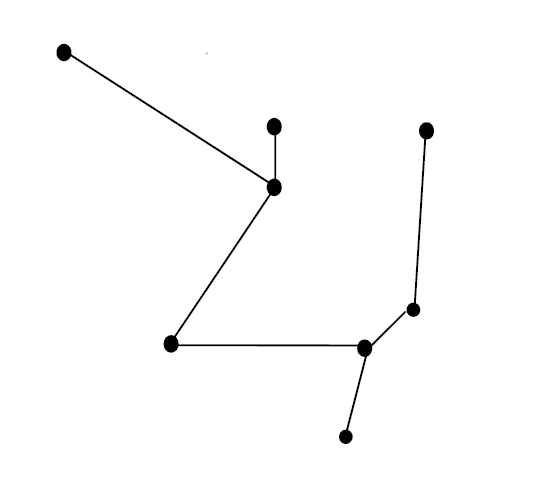
\includegraphics[scale=0.4]{01}
	\label{01}
\end{figure}


\end{frame}

\begin{frame}
\frametitle{Definição}
São equivalentes as seguintes proposições. Dado um grafo $G$:
\begin{enumerate}
	\item $G$ é uma árvore;
	\item $G$ é conexo e não tem ciclos;
	\item Entre cada par de vértices de $G$ existe um único caminho;
	\item $G$ é conexo com ordem $n$ e tamanho $n-1$;
	\item $G$ é conexo, mas $G-e$ não é conexo para todo aresta $e$ que pertence a $E(G)$ (conjunto das arestas);
	\item $G$ é acíclico, mas $G + uv$ contém um ciclo para todo par $u,v$ de vértices independentes.
\end{enumerate}

\end{frame}

\begin{frame}
\frametitle{Árvore Geradora}
{\bf Definição:} Uma árvore geradora de um grafo $G$ é um grafo que contém cada vértice de $G$ e é uma árvore.

\pause

{\bf Proposição:} \begin{enumerate}
	\item Cada grafo conexo tem uma árvore geradora;
	\item Duas árvores geradoras quaisquer um grafo têm a mesma quantidade de arestas.
\end{enumerate}

\end{frame}

\begin{frame}
\frametitle{Árvore Geradora}

Seja o grafo $G$ abaixo:

\begin{figure}[!h]
	\centering
	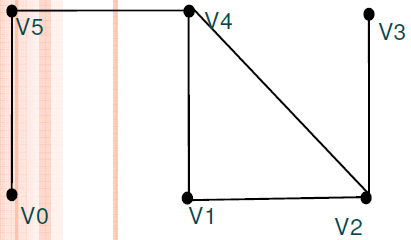
\includegraphics[scale=0.4]{02}
	\label{02}
\end{figure}

Este grafo possui o circuito $v_2 v_1 v_4 v_2$.

\end{frame}

\begin{frame}
\frametitle{Árvore Geradora}

Assim, todas as árvores geradoras são:

\begin{figure}[!h]
	\centering
	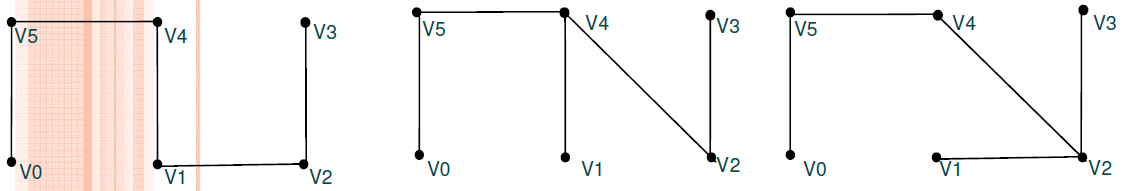
\includegraphics[scale=0.4]{03}
	\label{03}
\end{figure}

\end{frame}


\begin{frame}
\frametitle{Árvore Geradora}

Seja o grafo $G$:

\begin{figure}[!h]
	\centering
	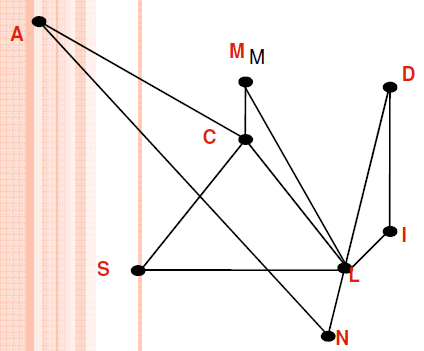
\includegraphics[scale=0.3]{04}
	\label{04}
\end{figure}

Um exemplo de árvore geradora é:

\begin{figure}[!h]
	\centering
	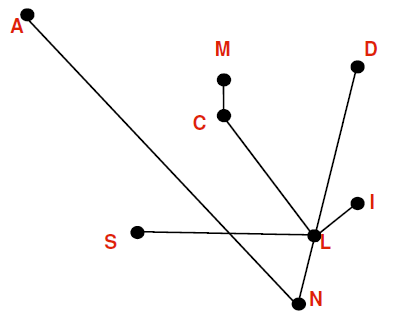
\includegraphics[scale=0.3]{05}
	\label{05}
\end{figure}


\end{frame}

\begin{frame}
\frametitle{Como encontrar uma Árvore Geradora?}

\begin{enumerate}
	\item Se o grafo $G$ não tem ciclos, então $G$ é uma árvore geradora;
	\item Se o grafo $G$ possui ciclos, é necessário remover recursivamente arestas (até determinar uma árvore), mantendo o grafo conectado.
\end{enumerate}

\end{frame}

\begin{frame}
\frametitle{Como encontrar uma Árvore Geradora?} 

\begin{figure}[!h]
	\centering
	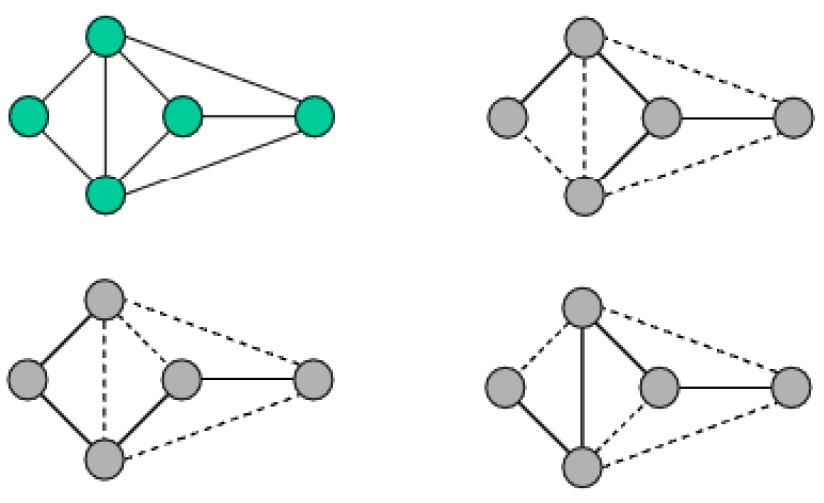
\includegraphics[scale=0.4]{06}
	\label{06}
\end{figure}

\end{frame}

\section{Árvore Geradora Mínima}

\begin{frame}
\frametitle{Minimal Spanning Tree (MST)}

\begin{enumerate}
	\item Em muitas das aplicações de relações com conexões simétricas. O grafo da relação modela uma situação na qual as arestas assim como os vértices carregam informação.
	\item O \emph{grafo ponderado} é um grafo no qual cada aresta é etiquetada com um valor numérico denominado peso.
\end{enumerate}
\end{frame}

\begin{frame}
\frametitle{Minimal Spanning Tree (MST)}

Cidade de “Oz” onde as trilhas do circuito de trens entre os pontos turísticos formam um grafo ponderado, os pesos indicam a distância em quilômetros.

\begin{figure}[!h]
	\centering
	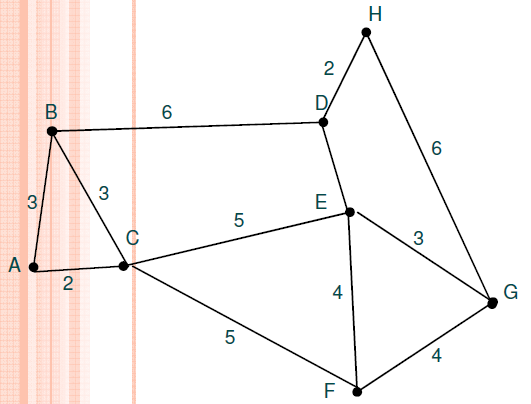
\includegraphics[scale=0.4]{07}
	\label{07}
\end{figure}

\end{frame}

\begin{frame}
\frametitle{Minimal Spanning Tree (MST)}
\begin{enumerate}
	\item Os pesos de uma aresta $(v_i, v_j)$ é algumas vezes referenciada como a distância entre vértices $v_i$ e $v_j$.
	\item Um vértice $u$ é um vizinho próximo do vértice $v$ se $u$ e $v$ são adjacentes e não há nenhum outro vértice unido a $v$ por uma aresta de peso menor do que $(u,v)$.
	\item Note que $v$ pode ter mais do que um vizinho próximo.
\end{enumerate}
\end{frame}

\begin{frame}
\frametitle{Minimal Spanning Tree (MST)}
{\bf Definição:} Um \emph{grafo com peso} é um grafo onde cada aresta possui um peso representado por um número real. A soma de todos os pesos de todas as arestas é o peso total do grafo.

Uma \emph{árvore geradora mínima} para um grafo com peso é uma árvore geradora que tem o menor peso total possível uma árvore geradora que tem o menor peso total possível dentre todas as possíveis árvores geradoras do grafo.

\pause

Se $G$ é um grafo com peso e $e$ é uma aresta de $G$, então:
\begin{enumerate}
	\item $w(e)$ indica o peso da aresta $e$;
	\item $w(G)$ indica o peso total do grafo $G$.
\end{enumerate}

\end{frame}


\begin{frame}
\frametitle{Minimal Spanning Tree (MST)}

Uma companhia aérea recebeu permissão para voar nas seguintes rotas.

O grafo de rotas da companhia aérea que recebeu permissão para voar pode ser “rotulado” com as distâncias entre as cidades:

\begin{figure}[!h]
	\centering
	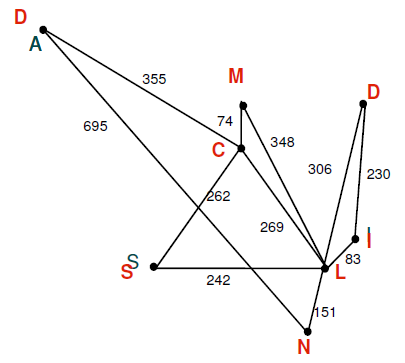
\includegraphics[scale=0.4]{08}
	\label{08}
\end{figure}


\end{frame}

\begin{frame}
\frametitle{Minimal Spanning Tree (MST)}

A companhia deseja voar para todas as cidades mas usando um conjunto de rotas que minimiza o total de distâncias percorridas:

\begin{itemize}
	\item Precisa-se determinar a árvore geradora;
	\item A árvore geradora deve ser mínima.
\end{itemize}

\begin{multicols}{2}
	\begin{figure}[!h]
		\centering
		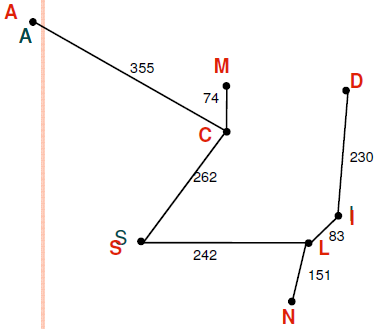
\includegraphics[scale=0.4]{09}
		\label{09}
	\end{figure}

	\begin{figure}[!h]
		\centering
		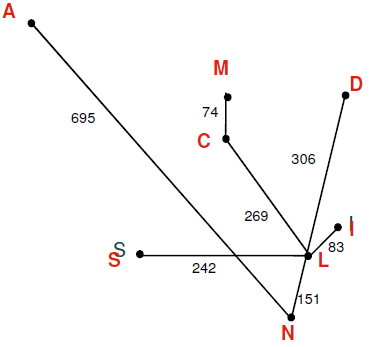
\includegraphics[scale=0.4]{10}
		\label{10}
	\end{figure}
\end{multicols}

\end{frame}

\section{Algoritmos para obter a Árvore Geradora Mínima}

\begin{frame}
\frametitle{Algoritmos para obter a Árvore Geradora Mínima}

Serão apresentados dois algoritmos:
\begin{itemize}
	\item Algoritmo de Prim;
	\item Algoritmo de Kruskal.
\end{itemize}

	\begin{figure}[!h]
	\centering
	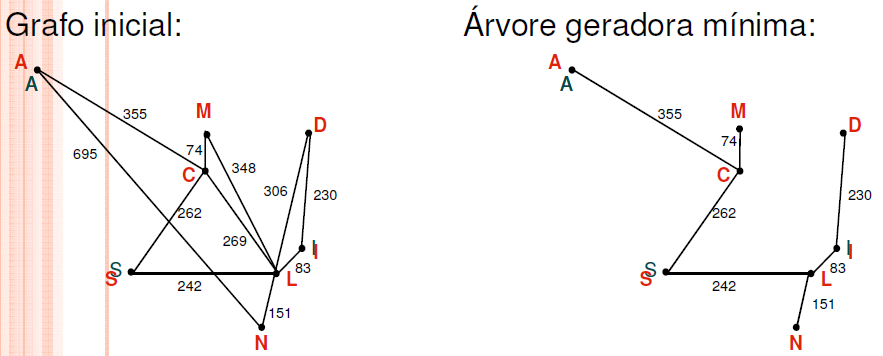
\includegraphics[scale=0.4]{11}
	\label{11}
	\end{figure}

\end{frame}

\begin{frame}
\frametitle{Algoritmo de Prim}

{\bf Ideia básica:}
\begin{itemize}
	\item Passo 01: Escolher o vértice $v_1$ de $G$.
	\\ Seja $V = \{v_1\}$ e $E = \{ \}$
	\item Passo 02: Escolher o vizinho próximo de $v_1$ de $V$ que seja adjacente a $v_1$, (por exemplo, $v_j \in V$) e para o qual a aresta $(v_1, v_j)$ não forma ciclo com os membros de $E$. Adicionar $v_j$ para $V$ e adicionar $(v_1, v_j)$ para $E$.
	\item Passo 03: Repetir $02$ até todos os vértices sejam visitados. Logo $V$ contém todos os vértices de $G$ e $E$ contém todas as arestas da $MST$ de $G$.
\end{itemize}

\end{frame}

\begin{frame}
\frametitle{Algoritmo de Kruskal}

{\bf Ideia básica:}
\begin{itemize}
	\item Passo 01: Ordenar as arestas por ordem crescente do comprimento (ou custo), sendo os desempates feitos arbitrariamente, formando uma lista.
	\item Passo 02: Selecionar a primeira aresta da lista.

	Se originar um ciclo, retirá-la da lista e voltar ao início do
	Passo 02.
	
	Caso contrário, adicioná-la à árvore e retirá-la da lista.
	\item Passo 03: Repetir o passo 2 até que a árvore esteja
	formada (todos os vértices conectados).
\end{itemize}
\end{frame}



\end{document}

